\chapter{ Características de Transferencia}

\section{Simulación}
\subsection{Simulación (JFET)}

\begin{figure}[H]
    \centering
    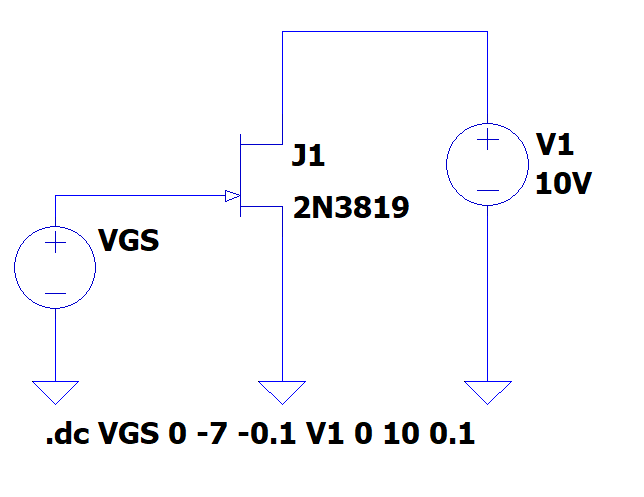
\includegraphics[width=0.5\textwidth]{img/circuito_tr.png}
    \caption{Descripción de la imagen.}
    \label{fig:imagen}
\end{figure}

\begin{figure}[H]
    \centering
    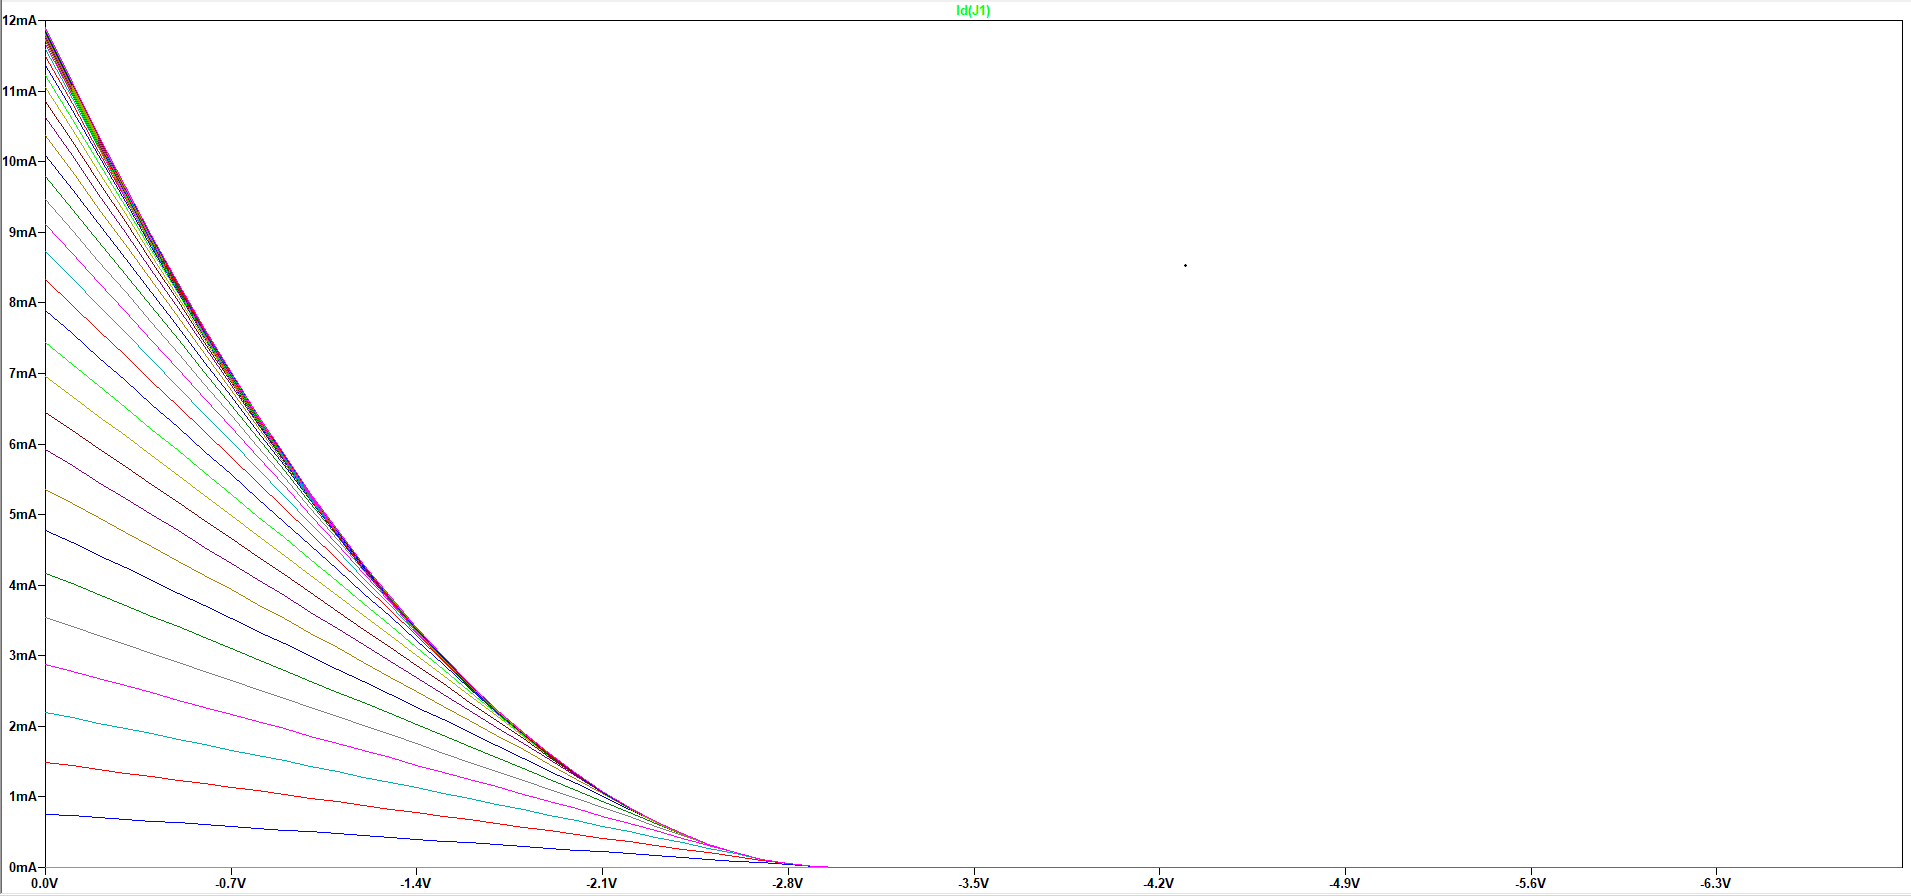
\includegraphics[width=\textwidth]{img/transf.png}
    \caption{Descripción de la imagen.}
    \label{fig:imagen}
\end{figure}

\subsection{ Simulación (MOSFET)}

\begin{figure}[H]
    \centering
    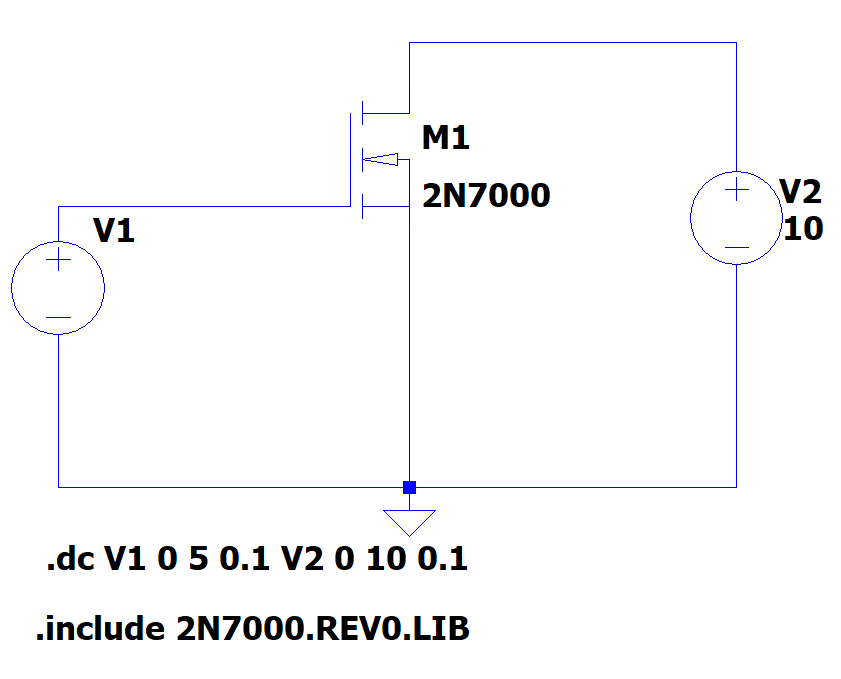
\includegraphics[width=0.5\textwidth]{img/circuito_tr_2N7000.png}
    \caption{Descripción de la imagen.}
    \label{fig:imagen}
\end{figure}


\begin{figure}[H]
    \centering
    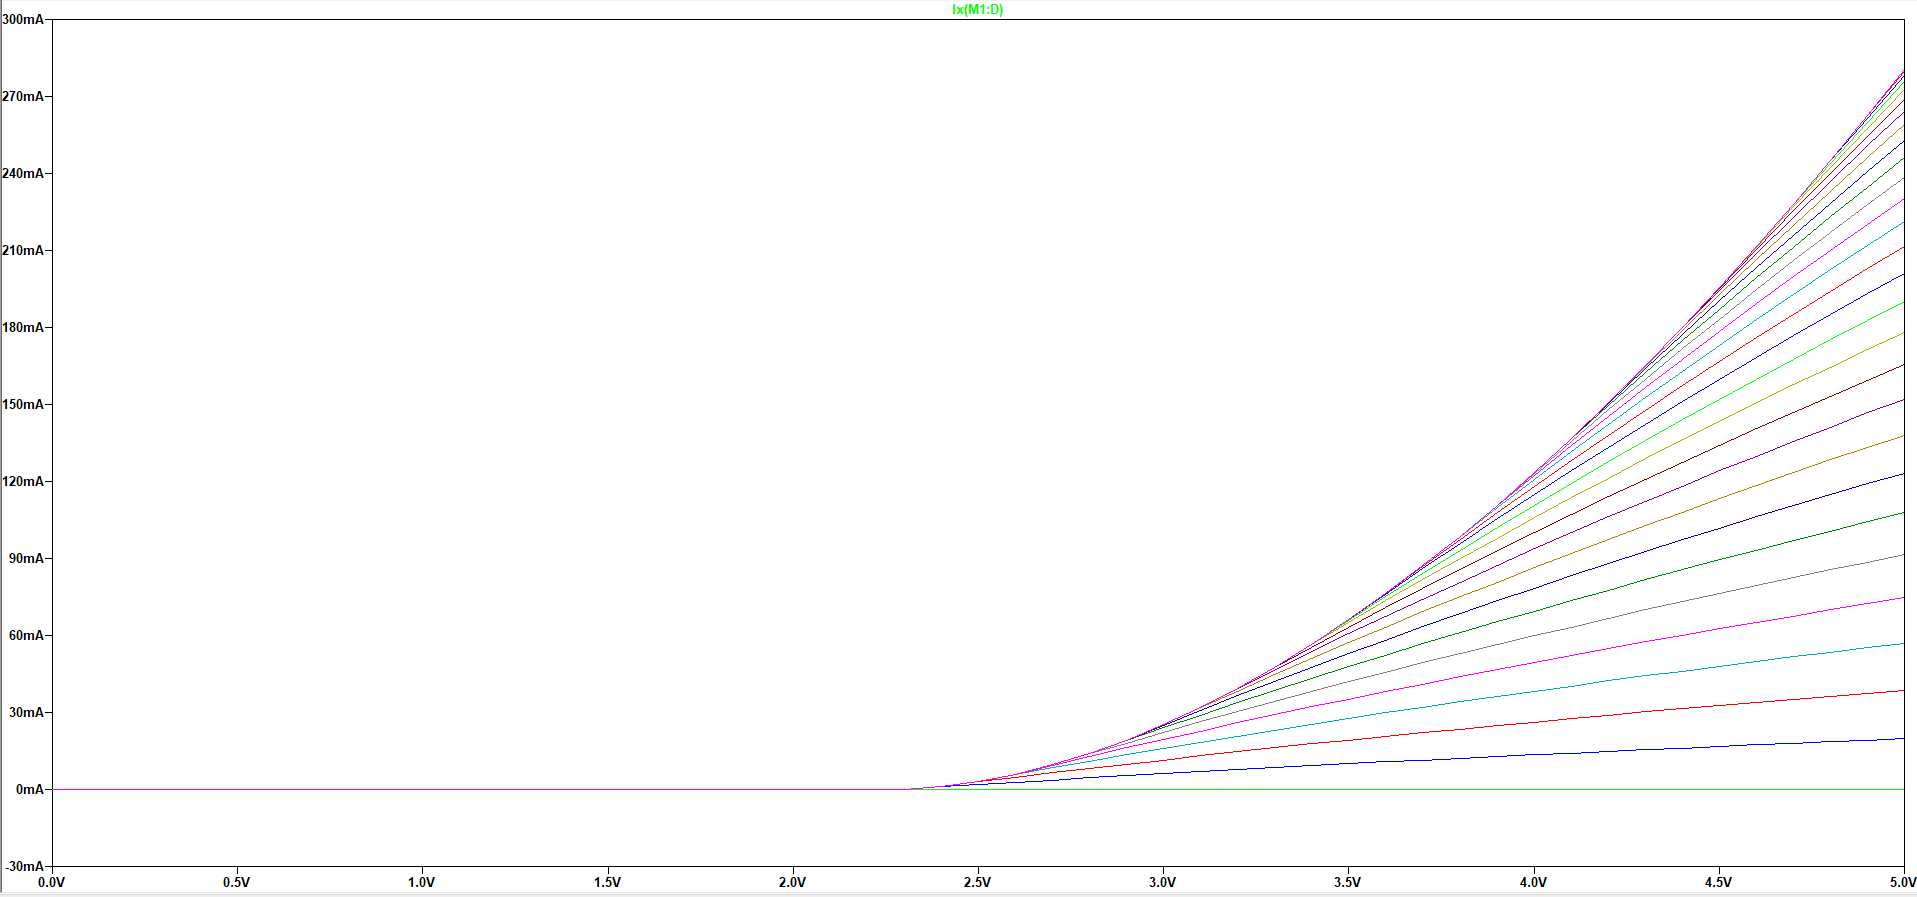
\includegraphics[width=\textwidth]{img/2N7000_TR.png}
    \caption{Descripción de la imagen.}
    \label{fig:imagen}
\end{figure}

\begin{table}[H]
    \centering
    \caption{Valores registrados para la obtención de la familia de curvas de transferencia $I_D=f(V_{GS})$.}
    \label{tab:curvas_transferencia}

    \begin{tabular}{|c|c|c|c|}
        \hline
        \shortstack{$V_{GS}$\\Medido [V]}&
        \shortstack{Curva 1\\
        $I_D$ [mA] $(V_{DS}=2\,\mathrm{V})$} &
        \shortstack{Curva 2\\
        $I_D$ [mA] $(V_{DS}=5\,\mathrm{V})$} &
        \shortstack{Curva 3\\
        $I_D$ [mA] $(V_{DS}=10\,\mathrm{V})$} \\
        \hline
        
        $0.0$ & & & \\ \hline
        $1.0$ & & & \\ \hline
        $1.5$ & & & \\ \hline
        $1.8$ & & & \\ \hline
        $2.0$ & & & \\ \hline
        $2.2$ & & & \\ \hline
        $2.4$ & & & \\ \hline
        $2.6$ & & & \\ \hline
        $2.8$ & & & \\ \hline
        $3.0$ & & & \\ \hline
        $3.5$ & & & \\ \hline
        $4.5$ & & & \\ \hline
        
    \end{tabular}
\end{table}




\begin{figure}[H]
    \centering
    
    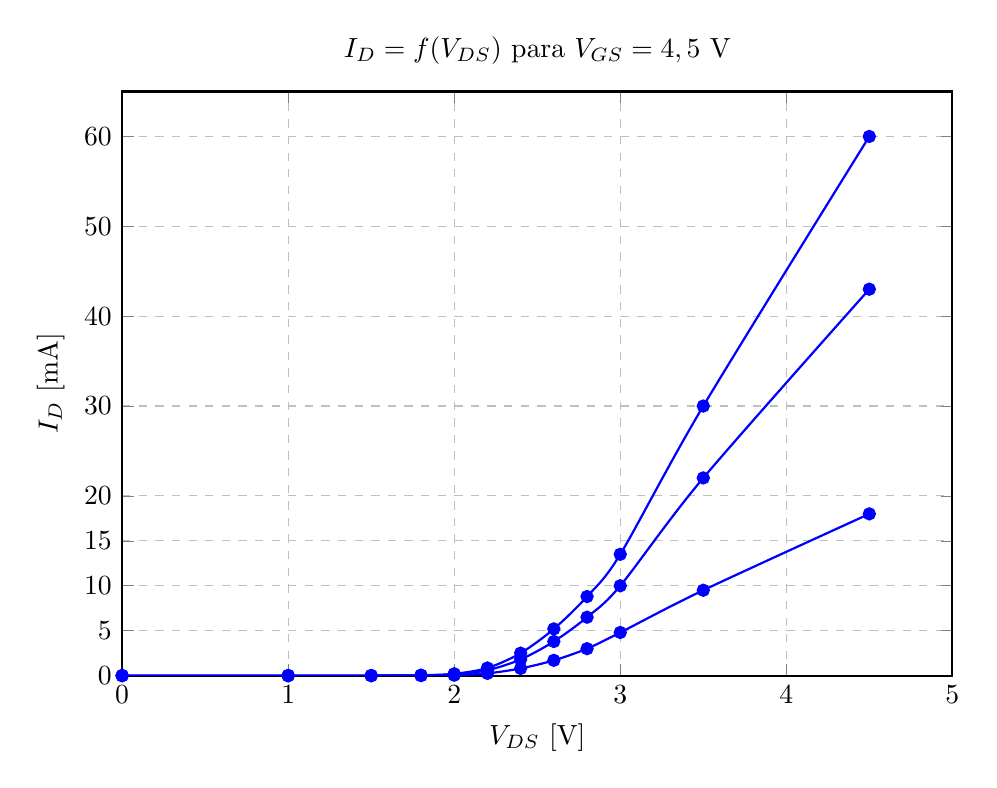
\begin{tikzpicture}
        \begin{axis}[
            width=\textwidth,
            height=9cm,
            xlabel={$V_{DS}$ [V]},
            ylabel={$I_D$ [mA]},
            title={$I_D=f(V_{DS})$ para $V_{GS}=4,5$ V},
            xmin=0, xmax=5,
            ymin=0, ymax=65,
            xtick={0,1,2,3,4,5},
            ytick={0,5,10,15,20,30,40,50,60,70},
            grid=both,
            minor grid style={dotted},
            major grid style={dashed},
            thick,
            mark size=2pt,
        ]
        
        \addplot[
            mark=*,
            smooth,
            thick,
            blue
        ] coordinates {
            (0,0)
            (1,0)
            (1.5,0)
            (1.8,0.01)
            (2,0.05)
            (2.2,0.25)
            (2.4,0.8)
            (2.6,1.70)
            (2.8,3)
            (3,4.80)
            (3.5,9.5)
            (4.5,18)
        };
        


        \addplot[
            mark=*,
            smooth,
            thick,
            blue
        ] coordinates {
            (0,0)
            (1,0)
            (1.5,0)
            (1.8,0.03)
            (2,0.15)
            (2.2,0.6)
            (2.4,1.8)
            (2.6,3.80)
            (2.8,6.5)
            (3,10)
            (3.5,22)
            (4.5,43)
        };
        
        
        \addplot[
            mark=*,
            smooth,
            thick,
            blue
        ] coordinates {
            (0,0)
            (1,0)
            (1.5,0)
            (1.8,0.04)
            (2,0.2)
            (2.2,0.85)
            (2.4,2.5)
            (2.6,5.20)
            (2.8,8.8)
            (3,13.5)
            (3.5,30)
            (4.5,60)
        };
        

        \end{axis}
    \end{tikzpicture}
    
    \caption{Curva experimental $I_D=f(V_{DS})$ para $V_{GS}=4,5$ V.}
    \label{fig:id_vds}
\end{figure}